\section{Slutord}
Vi i projektgruppen är nöjda med det resultat som vi har nått men är medvetna om
att det finns mycket att förbättra. Vi tycker kursen har varit bra, då den har
gett oss möjligheten att förbättra våra färdigheter inom elektronik inom ett
projekt som för oss varit både roligt och intressant. Vi hoppas att kursen även
i framtiden tillåter studenterna att fritt välja projekt, då vi tror att
projektet blir mer lärorikt när man får arbeta med ett projekt som man själv
valt utifrån intresse. Hur svävaren nu ser ut i verkligheten kan man se i figur
\ref{fig:theResult}.


\begin{figure}[htbp!]
\centering
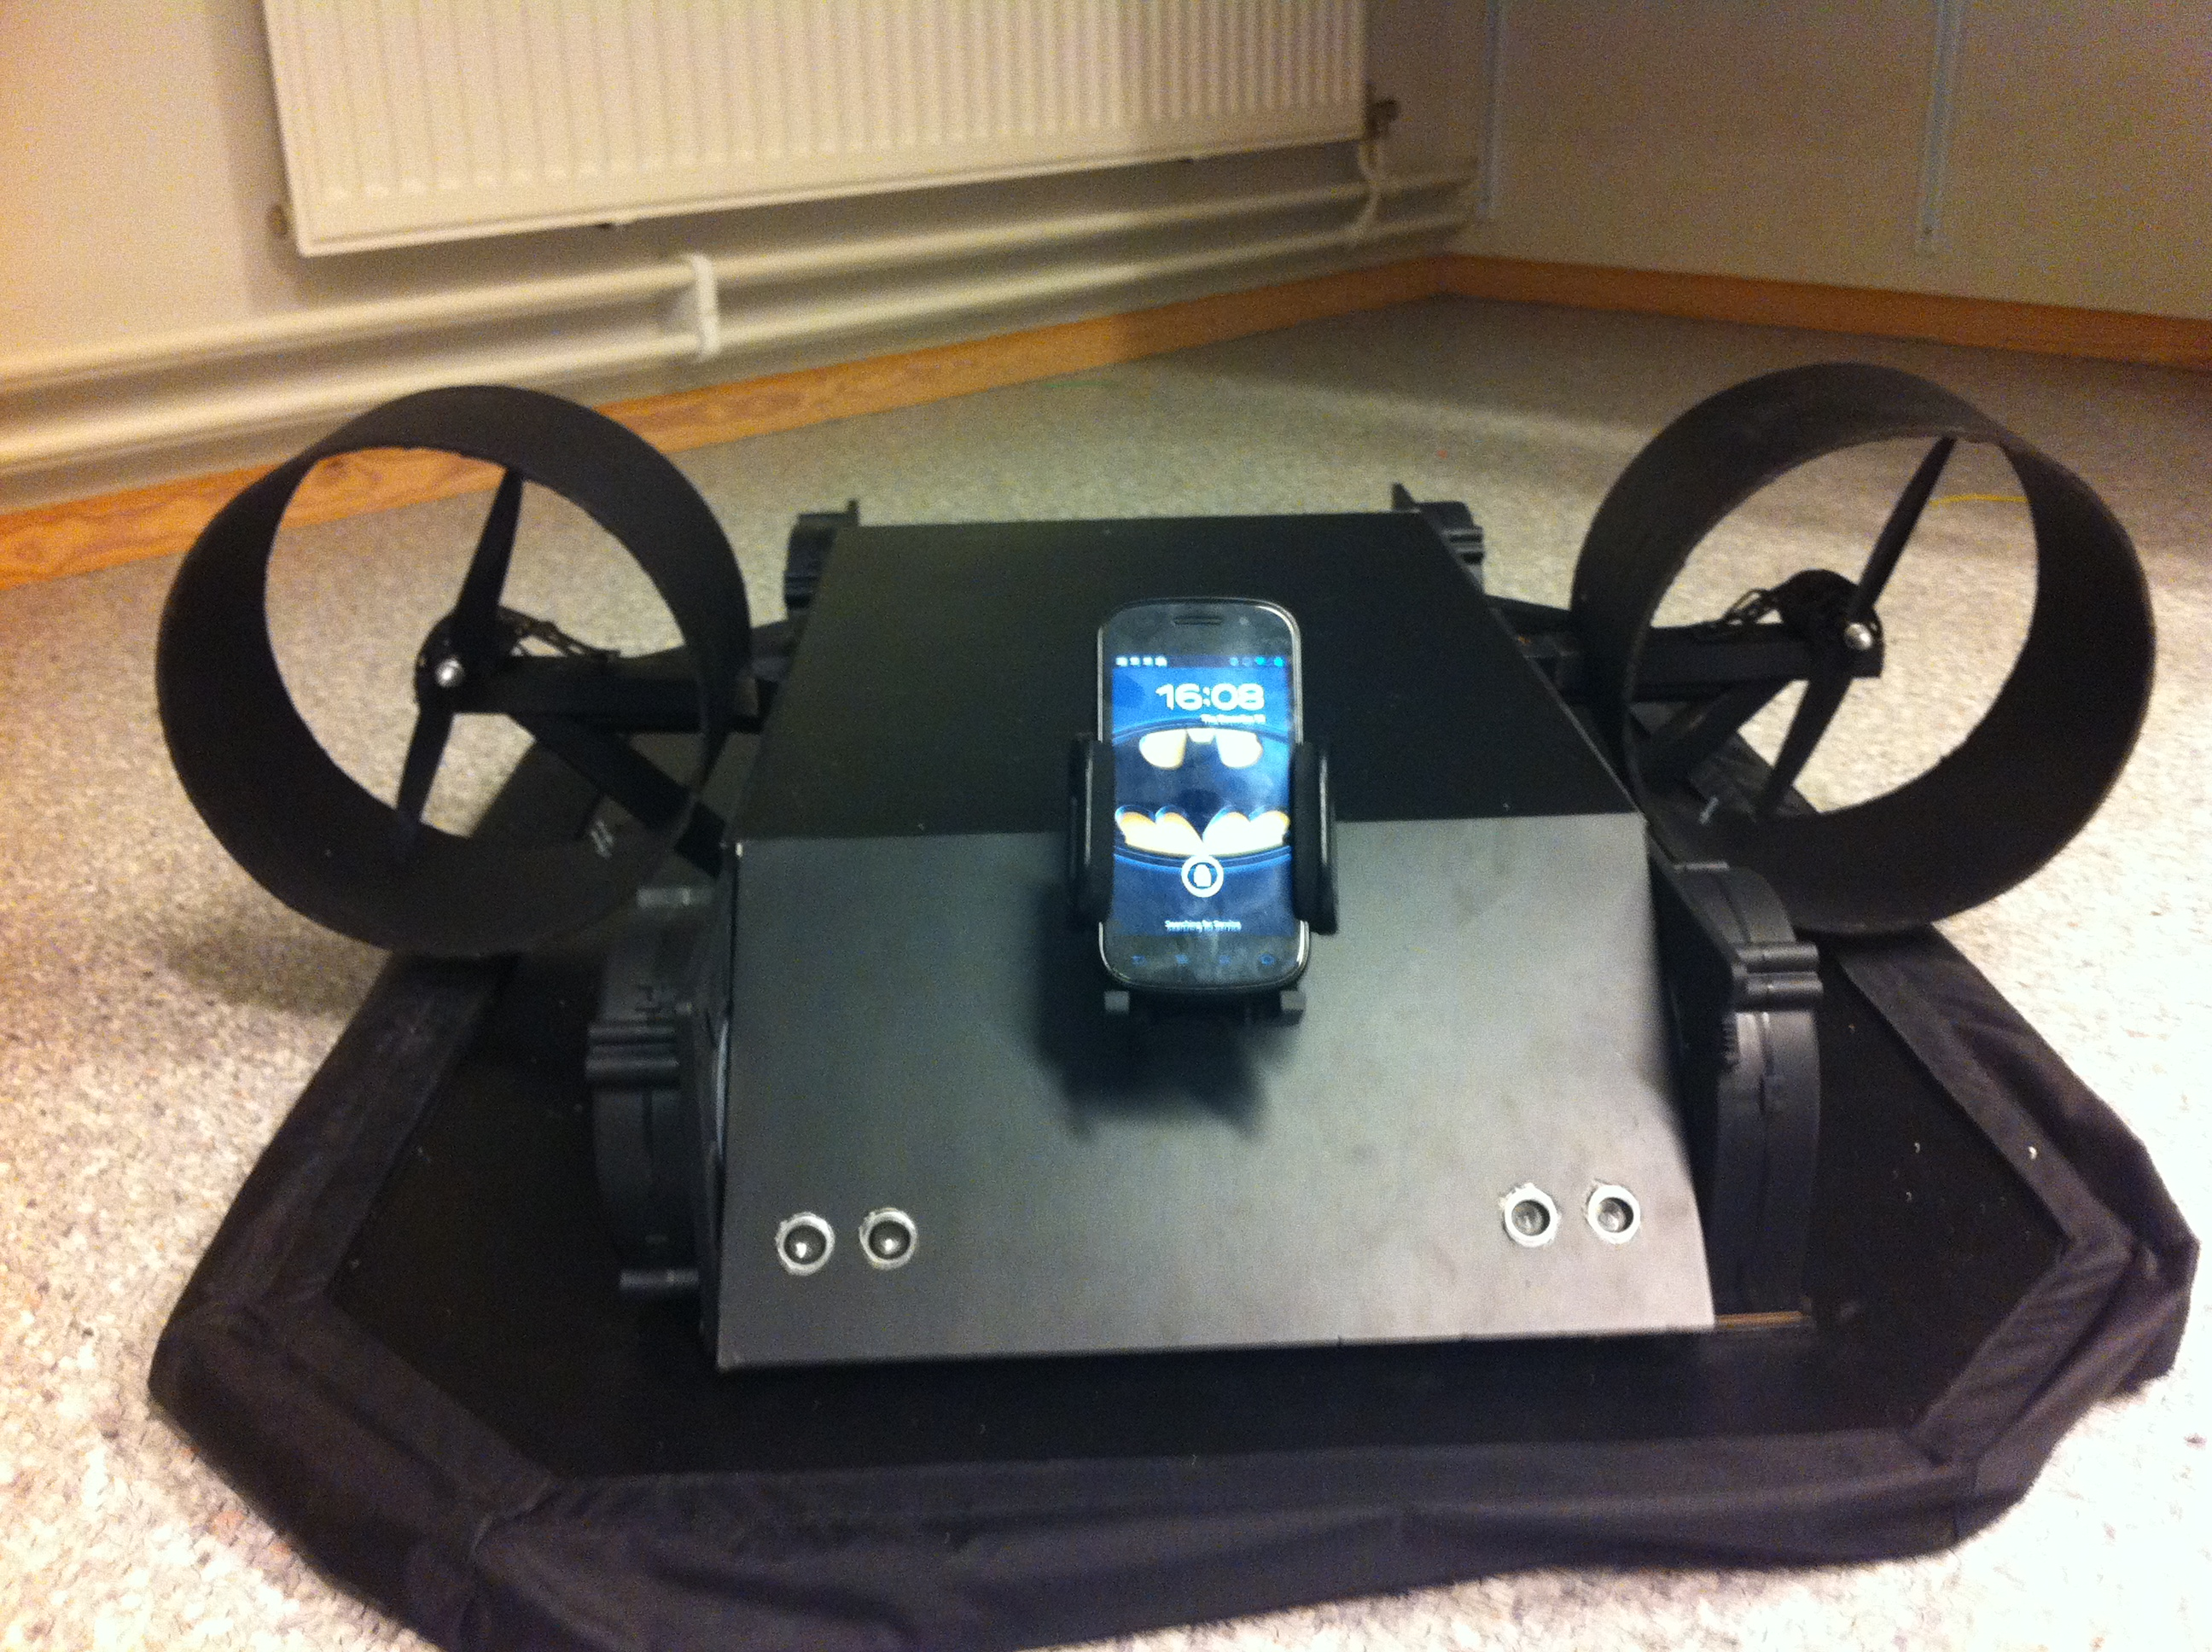
\includegraphics[width=12cm]{../../includes/figures/theResult}
\caption{Svävaren i sitt slutförande.}
\label{fig:theResult}
\end{figure}


Vi tror att svävaren som den är idag är en bra plattform som andra ED studenter
kan bygga vidare på i kommande års CDIO-projekt. Vi hoppas att den resulterande
svävaren kommer leva kvar inom ED så som den tidigare svävaren (framtagen 2008 i
deras robotkurs) har gjort. Om kommande års studenter inte vill bygga direkt på
denna svävare hoppas vi att de antar utmaningen och skapar en egen svävare och
testar sin egna design. Vi önskar kommande års studenter lycka till i deras
CDIO-projekt, oavsett om de väljer att bygga vidare på vår plattform, skapa en
egen svävare eller göra något helt annat och hoppas att deras projekt blir lika
roligt och lärorikt som vårt varit.

Projektgruppen vill även tacka Norrköpings Polytekniska Förening för utdelat
stipendium. Utan detta hade det inte varit möjligt att genomföra projektet.
Projektgruppen vill också tacka Björn-Åke Sköld för hjälp och material vid
konstruktionen av den mekaniska delen av projektet.

Vi vill även tacka institutionen ITN för upplåtandet av laborationssal en hel
termin för detta projekt. Det har underlättat otroligt att ha en stor och
välutrustad sal till förfogande vid detta stora utvecklingsprojekt.

Avslutningsvis så vill projektgruppen även tacka Tomas Tranströmer för underbara
dikter som har förgyllt varje projektgruppsmöte. För att tolka metaforerna i
Tranströmers dikt Storm så kan man likna den utvecklade svävaren med den gamla
jätteeken, där alla de möjligheter för utvecklingsuppgifter beskrivs som en
förstenad älgs milsvida krona.
